\documentclass[11pt,a4paper]{article}
\usepackage[T1]{fontenc}
\usepackage[utf8]{inputenc}
\usepackage{lmodern,microtype}
\usepackage[margin=25mm,headheight=14pt]{geometry}
\usepackage{amsmath,amssymb,amsthm}
\usepackage{booktabs,tabularx,array,longtable}
\usepackage[font=small,labelfont=bf,justification=raggedright,singlelinecheck=false]{caption}
\usepackage{enumitem,xcolor,fancyhdr,fvextra}
\usepackage{tikz}
\usetikzlibrary{arrows.meta,positioning}
\usepackage{xurl}
\usepackage[hidelinks,pdfusetitle]{hyperref}
\usepackage{bookmark}
\definecolor{ink}{HTML}{17334C}
\definecolor{accent}{HTML}{236F78}
\definecolor{pale}{HTML}{EDF4F5}
\hypersetup{colorlinks=true,linkcolor=ink,citecolor=accent,urlcolor=accent}
\pagestyle{fancy}
\fancyhf{}
\fancyhead[L]{\small K215 proof simplification}
\fancyhead[R]{\small Pinned-source proposal}
\fancyfoot[C]{\thepage}
\setlength{\parskip}{0.35em}
\setlength{\parindent}{0pt}
\setlength{\emergencystretch}{2em}
\setlist{topsep=3pt,itemsep=3pt,parsep=0pt}
\renewcommand{\arraystretch}{1.15}
\newcolumntype{Y}{>{\raggedright\arraybackslash}X}
\newcommand{\code}[1]{\texttt{\detokenize{#1}}}
\newcommand{\repo}{https://github.com/VladimirReshetnikov/ProveIt}
\newcommand{\pin}{cbf94cb552a3b49509e0eee80e7455d4eb5974c6}
\newcommand{\src}[2]{\href{\repo/blob/\pin/#1}{#2}}
\newcommand{\Halts}{\operatorname{Halts}}
\newcommand{\Con}{\operatorname{Con}}
\newcommand{\some}{\operatorname{some}}
\newcommand{\none}{\operatorname{none}}
\newcommand{\Reach}{\operatorname{Reach}}
\newcommand{\reads}{\operatorname{reads}}
\newcommand{\eval}{\operatorname{eval}}
\newcommand{\ZFC}{\mathsf{ZFC}}
\newcommand{\ZF}{\mathsf{ZF}}
\newtheorem{theorem}{Theorem}[section]
\newtheorem{lemma}[theorem]{Lemma}
\theoremstyle{remark}
\newtheorem{remark}[theorem]{Remark}
\title{\vspace{-1.2cm}\color{ink}\textbf{Simplifying the K215 Correctness Proofs}\\[0.45em]
\large Native Replacement, Shared Runtime Contracts,\\and Clock-Free Termination}
\author{Technical proposal for Vladimir Reshetnikov's ProveIt repository\\
\small Prepared with ChatGPT; source audits and checked component prototypes}
\date{22 October 2026}
\hypersetup{pdftitle={Simplifying the K215 Correctness Proofs},
pdfauthor={Technical proposal for the ProveIt repository}}
\begin{document}
\maketitle
\begin{abstract}
The current K215 endpoint is already a small composition of substantial shared
theorems. Further simplification should target redundant semantic constructions,
duplicated runtime implementations, and the induction interfaces used by their
clients. We give three concrete proposals against a pinned repository revision.
First, a checked Lean patch derives Replacement from the quotient's existing
Collection theorem and separates a generic module from its legacy
specializations. It reduces the literal endpoint's static project-source closure
by 165 physical lines and 8,358 bytes, while retaining every old interface.
Second, an audit identifies 318,724 bytes in seven additional copies of five
Rocq runtime modules; a checked finite-support transport prototype specifies a
sound reuse boundary, but the common runtime refactor remains to be implemented.
Third, a checked Lean adapter replaces clock subtraction in the current
simulation theorem with induction over reachable suffixes. Its client is shorter,
but the new library has a net source cost for a single client.

The report distinguishes source size, proof architecture, assumption profiles,
and completed verification. These are component-level improvements, not a fresh
full-machine certification or an internal derivation in ZFC.
\end{abstract}
\begingroup\setlength{\fboxsep}{8pt}
\colorbox{pale}{\parbox{\dimexpr\linewidth-2\fboxsep\relax}{
\textbf{Recommended order.}
Integrate native Replacement and its import split first. Port the existing
Lean table-parametric runtime boundary to Rocq next. Adopt the termination
library separately when additional clients justify its maintenance cost.
The exact 215-state machine, source program, and consistency statement are
preserved by the supplied Lean proposals.}}
\endgroup
\vspace{0.6em}

\textbf{Source pin:} \href{\repo/commit/\pin}{\texttt{\pin}}.
All repository references below use this immutable revision. Source counts
include comments and blank lines unless explicitly stated otherwise.
\clearpage
\begingroup
\small
\setlength{\parskip}{0pt}
\tableofcontents
\endgroup
\clearpage

\section{The target and the current baseline}
\label{sec:baseline}
\subsection{What must be preserved}
For the accepted literal K215 machine \(M_{215}\), the formal endpoint is
\begin{equation}
  \Halts(M_{215},\mathrm{blank})
  \quad\longleftrightarrow\quad
  \text{there is a finite ZFC derivation of falsity}.
  \label{eq:endpoint}
\end{equation}
Negating both sides gives nonhalting if and only if syntactic
\(\Con(\ZFC)\). No consistency assumption is a premise of this equivalence.
The intended application is a machine whose behavior expresses the consistency
question; no simplification here claims unconditional nonhalting or a smaller
state count.

The repository identifies a specific dense table: 215 working states, two
symbols, one two-way infinite tape, blank input, initial state 0, and a separate
halt. Initialization is included in the state count. Both maintained proof
lanes target this same table, rather than merely two machines of the same size
\cite{verification,endpoint215}.

There is a distinction relevant to the user's phrase \emph{provably equivalent
in ZFC}. The repository's verification statement explicitly describes
external Lean and Rocq theorems and says that an internal PA proof or a
derivation encoded in ZFC's own proof syntax is not supplied
\cite{verification}. This report preserves that status. It does not turn an
external proof-assistant theorem into an internally certified ZFC derivation
by changing its presentation. Section~\ref{sec:internal} explains the remaining
interface.

\subsection{Fresh source measurements}
The report's read-only census follows imports from
\code{BusyBeaver.ZFC.KEndpoint215}, resolves project modules through the
declared source roots in \code{lakefile.toml}, and excludes the Lean toolchain's
\code{Init}, \code{Std}, and \code{Lean} sources. It records the hash and import
list of every selected source. These are \emph{syntactic import-closure}
measurements; they are not counts of declarations actually referenced in the
final proof term.

\begin{table}[ht]
\centering\small
\begin{tabularx}{\linewidth}{Y r}
\toprule
Pinned-source observation & Value\\
\midrule
Project modules in the literal Lean endpoint closure & 174\\
UTF-8 bytes in that closure & 1,752,650\\
Physical lines in that closure & 37,648\\
Physical lines in \code{KEndpoint215.lean} itself & 54\\
Rocq \code{coq/215/} files / physical lines & 44 / 8,026\\
Dense machine actions & 430\\
Expanded source leaves & 4,751\\
Guarded site outcomes, counting both decrement cases & 6,176\\
Maximum expanded source depth / checker bound & 47 / 48\\
\bottomrule
\end{tabularx}
\caption{Current-source counts. The machine and source counts are reproduced
in \code{evidence/baseline-census.json}; the Rocq counts are in
\code{rocq-runtime/runtime_audit.json}.}
\end{table}

The leaf counts are 1,900 increments, 1,425 decrements, 1,327 continues,
98 breaks, and one halt. The literal bootstrap has 95,714 steps; its
representation uses gap 65 and 40 spare register blocks. These are identity
and boundary facts, not proposed optimization targets
\cite{boot215,endpoint215,sites215}.

The repository's phase-15 summary reports an earlier 176-module closure.
Subsequent changes are present at the pin used here. Comparing the proposed
overlay against that historical figure would mix baselines. The fresh
174-module census is the baseline for every closure reduction in this report.

\subsection{Substantial simplifications already exist}
The maintained proof already has the principal architecture one might suggest
on a first reading: a generic K-family endpoint, positive-progress simulation,
machine-specific finite certificates, and a shared logical calibration
\cite{endpoint,ksim,history}. In particular:
\begin{itemize}
\item The final Lean theorem instantiates a shared composition with dense
renaming, register-engine contracts, boot reachability, site coverage, and
source correctness.
\item The source correspondence uses a normalized 1,426-entry certificate.
The reverse direction is recovered from symmetry of the checked bisimulation,
rather than
proved by a separate equally large certificate.
\item The current lower semantic chain constructs the seed property on the
original model and shares quotient syntax and recursion infrastructure.
\item The source tree is already computed from the source program.
Replacing the former large literal tree by that definition is not a new
opportunity at this pin.
\item Rocq's final source and correctness files are already short facades.
Recent commits have also removed unused initial-state enumerator theorems and
shared paired dispatch tactic scripts.
\end{itemize}
Accordingly, the proposals below concentrate on changes that remain useful at
the current revision. The guarded-image and reachable-suffix ideas also occur
in the repository's earlier proposal packets. The contribution here is
current-source integration, exact dependency accounting, explicit obligations,
and fresh component checks, not priority for those ideas
\cite{native-prior,collection-prior,further-prior,proof-core-prior}.

\section{Recommendation and expected benefit}
\begin{table}[ht]
\centering\small
\begin{tabularx}{\linewidth}{@{}p{0.19\linewidth} Y Y@{}}
\toprule
Change & Completed result & Benefit and limit\\
\midrule
Native Replacement &
Current Lean overlay, compatibility clients, generic endpoint compilation &
Active closure: \(-165\) lines, \(-8{,}358\) bytes.
All maintained affected sources: \(+84\) lines.\\
\addlinespace
Shared Rocq runtime &
Eight-variant census; kernel-checked adaptive-query transport and K215/K217
support witness &
318,724 bytes in seven extra copies of five modules. This is a duplication
inventory, not an achieved net saving.\\
\addlinespace
Termination transport &
Generic Lean theorem, exact adapters, actual \code{KSim} patch,
checked counterexamples &
Client file: \(-28\) lines. Client plus new library: \(+188\) lines.
Best treated as a shared abstraction.\\
\bottomrule
\end{tabularx}
\caption{Three separately evaluated changes. Their metrics must not be added
as though a combined full endpoint build had been performed.}
\end{table}
The semantic change is the first adoption candidate because it removes an
entire repeated style of reasoning from the active proof: representative
selection, bisimulation invariance, and quotient descent for Replacement.
The Rocq consolidation is the larger maintenance opportunity because changing a
shared runtime theorem should require changing one proof. The termination
abstraction improves local reasoning, but its source cost makes it a secondary
recommendation.

The common principle is to prove a semantic property at the layer where its
natural equality and invariants are already available. It is usually more
valuable to remove a second proof route than to shorten individual tactic
scripts within both routes.

\section{Native Replacement after quotient Collection}
\label{sec:native}
\subsection{The existing route repeats quotient work}
\code{KQ1Collect.quotient_collection} already supplies Collection for every
actual first-order formula, with arbitrary parameter valuations in the
quotient model. Its proof has already handled representative lifting and
the equivalence relation on raw objects \cite{collect}.

The current \code{KQ1Replacement} independently introduces a guarded raw
matrix, proves its invariance, obtains interpreted Replacement, and descends
the resulting image to the quotient \cite{oldreplacement}. That is a valid
route, and its public helpers may remain useful. But the active native model
already has the interface needed for a much shorter argument:
Collection with literal equality.

The proposed route is
\[
 \text{quotient Collection}
 \ \Longrightarrow\
 \text{guarded functional image}
 \ \Longrightarrow\
 \text{native Replacement}.
\]
The new production file is only 74 physical lines, including the formula
adapter and both quotient wrappers. The elementary image lemma itself is
independent of the set-theoretic construction.

\subsection{The exact Collection contract}
It is essential to use the repository's actual contract
\cite{profilecollection}. For a membership relation \(m\), write \(x\in a\)
for \(m(x,a)\). For a binary relation \(r\), the proposition
\(\operatorname{ImageCollection}(r,a,b)\) is
\begin{align}
 &\forall y\in b\;\exists x\;r(x,y), \label{eq:support}\\
 &\forall x\in a\;
   \bigl((\exists y\;r(x,y))\ \Longrightarrow\
         \exists y\in b\;r(x,y)\bigr). \label{eq:coverage}
\end{align}
Collection for \(r\) means that such a \(b\) exists for every \(a\).
The support clause~\eqref{eq:support} does \emph{not} restrict its witness
\(x\) to the particular domain \(a\). This makes the domain guard necessary.
An unguarded application followed by functionality does not prove exact
image membership.

\begin{lemma}[Guarded functional image]
\label{lem:image}
Let \(r_a(x,y)\) abbreviate \(x\in a\land r(x,y)\).
Suppose Collection holds for \(r_a\), and suppose \(r\) is partially
functional on \(a\):
\[
 x\in a\land r(x,y)\land r(x,z)\ \Longrightarrow\ y=z.
\]
Then there is a \(b\) such that
\[
 y\in b \quad\longleftrightarrow\quad
 \exists x\;(x\in a\land r(x,y)).
\]
\end{lemma}
\begin{proof}
Apply Collection for \(r_a\) at domain \(a\), obtaining \(b\).
If \(y\in b\), the support clause gives \(x\) with
\(r_a(x,y)\), hence \(x\in a\land r(x,y)\).

Conversely, let \(x\in a\) and \(r(x,y)\). Coverage for \(r_a\) supplies
\(z\in b\) with \(x\in a\land r(x,z)\). Functionality gives \(z=y\),
so \(y\in b\).
\end{proof}
This proof requires neither totality of \(r\) on \(a\), nor extensionality,
nor an inhabited carrier, nor a choice principle. The checked Lean
\code{exact_image} theorem reports no axioms. Partial functionality is enough:
inputs with no output make no contribution to the image.

The finite examples in \code{scripts/check_guard_examples.py} illustrate
the necessity of the hypotheses. With
\(a=\{0\}\), \(r=\{(0,0),(1,1)\}\), the unguarded collection
\(b=\{0,1\}\) satisfies global support and coverage, but has an unwanted
member. Without functionality, \(r=\{(0,0),(0,1)\}\) permits the covering
set \(\{0\}\), which misses an output. Without support, coverage permits
extra members. These finite examples explain the interface; the general
result is proved in Lean, not inferred from the examples.

\subsection{Formula indexing and variable order}
The model supplies Collection for formulas, not arbitrary semantic predicates.
The generic mathematical relation \(r_a\) must therefore be realized by an
actual formula. The two existing APIs use different variable conventions:
\begin{center}\small
\begin{tabularx}{\linewidth}{@{}p{0.33\linewidth} p{0.25\linewidth} Y@{}}
\toprule
API & Slots 0 and 1 & Remaining slots\\
\midrule
\code{relOf phi env y x} & output \(y\), input \(x\) & original parameters\\
\code{MatrixRelation} & input \(x\), output \(y\) & collection parameters\\
Guarded matrix & input \(x\), output \(y\) & domain \(a\), then parameters\\
\bottomrule
\end{tabularx}
\end{center}
Define a renaming \(\rho:\mathbb N\to\mathbb N\) by
\[
 \rho(0)=1,\qquad \rho(1)=0,\qquad \rho(k+2)=k+3.
\]
The concrete guard is
\[
 \operatorname{guardForm}(\varphi)
   := \operatorname{Mem}(0,2)\land\operatorname{rename}(\rho,\varphi).
\]
In the environment \((x,y,a,\mathrm{env})\), its semantics is exactly
\[
 x\in a\ \land\ \operatorname{relOf}(m,\varphi,\mathrm{env},y,x).
\]
The supplied \code{sat_guardForm} proves this identity using the maintained
renaming theorem. Applying Collection to this formula and to the parameter
environment \((a,\mathrm{env})\) supplies the premise of
Lemma~\ref{lem:image}. The result is then converted by the existing
\code{bridge_Repl} to satisfaction of the usual Replacement schema.

This adapter does not introduce Collection for every semantic predicate.
Every call uses one concrete \code{Form}. The original \code{QHyp}
assumptions are unchanged. There is no second equality-free translation:
the quotient Collection theorem already interprets native equality.

\subsection{The import split is part of the proof simplification}
\label{sec:imports}
Replacing only \code{KQ1ZF}'s direct call is insufficient. The old development
remains in its transitive imports through
\[
 \code{KQ1ZF}
 \longrightarrow \code{InductiveAttempts}
 \longrightarrow \code{QuotientReplacement}
 \longrightarrow \code{KQ1Replacement}.
\]
The intermediate finite-attempt module contains a generic argument followed
by CP/GIC specializations. Only the specializations require the old quotient
Replacement interface \cite{attempts}.

The patch separates these parts at their existing boundary:
\begin{description}[style=nextline,leftmargin=0pt,labelwidth=0pt,labelsep=0pt]
\item[\code{InductiveAttemptsCore.lean}]
The generic finite-attempt development, with its original proof bodies
unchanged. It has no dependency on the legacy Replacement specialization.
\item[\code{InductiveAttempts.lean}]
A compatibility facade importing the core and retaining the original
specialization tail. Old declarations and module imports remain available.
\item[\code{KQ1ZF.lean}]
Imports the core and the new native Replacement module. Its Replacement
field and its call to \code{ordinary_infinity_of_container} receive the
new native theorem.
\end{description}

\begin{figure}[ht]
\centering
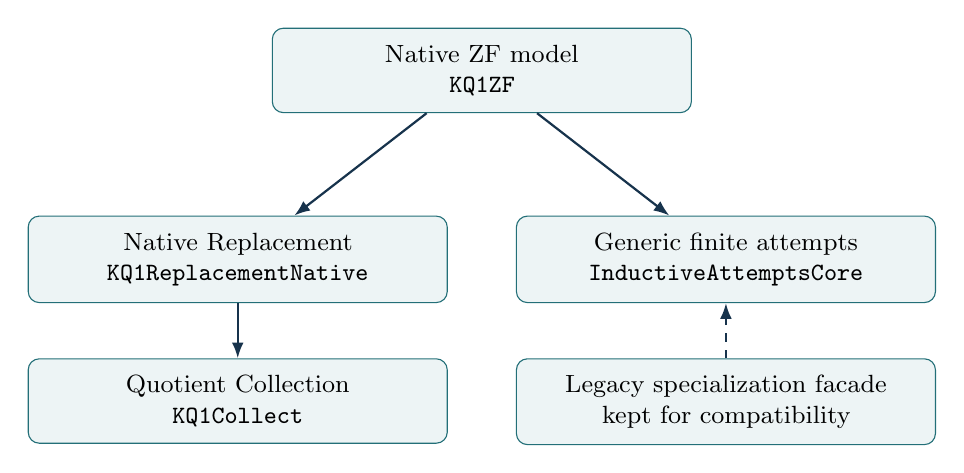
\begin{tikzpicture}[
  node distance=7mm and 9mm,
  box/.style={draw=accent,rounded corners,fill=pale,
     align=center,font=\small,inner sep=6pt,text width=49mm},
  arr/.style={-{Latex[length=2mm]},thick,draw=ink}]
 \node[box] (zf) {Native ZF model\\\texttt{KQ1ZF}};
 \node[box,below=13mm of zf,xshift=-31mm] (nat) {Native Replacement\\\texttt{KQ1ReplacementNative}};
 \node[box,below=13mm of zf,xshift=31mm] (core) {Generic finite attempts\\\texttt{InductiveAttemptsCore}};
 \node[box,below=of nat] (coll) {Quotient Collection\\\texttt{KQ1Collect}};
 \node[box,below=of core] (legacy) {Legacy specialization facade\\kept for compatibility};
 \draw[arr] (zf)--(nat);
 \draw[arr] (zf)--(core);
 \draw[arr] (nat)--(coll);
 \draw[arr,dashed] (legacy)--(core);
\end{tikzpicture}
\caption{Proposed dependency boundary. Arrows indicate imports or use of the
corresponding proof interface. The compatibility facade imports the core; the
active model does not import the facade.}
\end{figure}
The source-split audit checks byte-for-byte preservation of both the generic
and specialization proof bodies, and confirms that the old
\code{KQ1Replacement} and \code{QuotientReplacement} files are unchanged.
This is a modest structural edit, rather than a rewrite of the infinity proof.

The change is intentionally limited to Replacement. Existing collection
infrastructure uses separation-related valuation lifting, and the power
construction still needs raw subdomain reasoning. Moving every construction
to the native model at once would risk a dependency cycle or merely recreate
an auxiliary raw construction under a new name. The supplied patch makes no
such additional change.

\subsection{Measured effect and compatibility}
\begin{table}[ht]
\centering\small
\begin{tabular}{@{}lrrr@{}}
\toprule
Literal endpoint source closure & Baseline & Proposed & Difference\\
\midrule
Project modules & 174 & 173 & \(-1\)\\
UTF-8 source bytes & 1,752,650 & 1,744,292 & \(-8,358\)\\
Physical lines & 37,648 & 37,483 & \(-165\)\\
\bottomrule
\end{tabular}
\caption{Native Replacement plus the necessary import split. These are
independently reproduced static import counts.}
\end{table}
The active closure loses \code{InductiveAttempts},
\code{QuotientReplacement}, and \code{KQ1Replacement}, and gains
\code{InductiveAttemptsCore} and \code{KQ1ReplacementNative}.
Changing only the direct Replacement call would instead add one module,
3,544 bytes, and 74 lines to the active closure, because the old chain would
remain imported.

Compatibility has a real cost. Across all affected maintained production
files, including the retained facade and old proofs, this patch adds
3,902 bytes and 84 physical lines. It therefore simplifies and shrinks the
active endpoint closure; it does not reduce total repository source.
Legacy helper deletion could be considered after auditing all clients, but
no such deletion or additional saving is assumed here.

The old nine-declaration Replacement API and the finite-attempt
specializations are checked by a separate audit client. The two old and new
Replacement endpoints have identical proposition types. An audit equality
proved by \code{rfl} uses Lean proof irrelevance: it verifies type
compatibility, not identical proof algorithms, proof-term sizes, or
elaboration cost.

\section{A shared Rocq runtime for the K family}
\label{sec:rocq}
\subsection{The duplication is measurable}
The Rocq extension currently keeps physically separate variant directories
for K215, K217, K218, K221, K225, K226, K227, and K229.
The supplied audit removes nested comments, normalizes only namespace tokens
of the form \code{K<digits>F}, and removes blank lines and line-edge
whitespace. Under exactly this normalization, each of the following modules
has one common body across all eight variants.
\begin{table}[ht]
\centering\small
\begin{tabular}{@{}lrrr@{}}
\toprule
Module & Eight copies & K215 copy & Other seven\\
\midrule
\code{Zip} & 30,923 & 3,959 & 26,964\\
\code{Runtime230Core} & 156,227 & 19,622 & 136,605\\
\code{Tape230Blocks} & 69,539 & 8,786 & 60,753\\
\code{Tape230Carry} & 43,883 & 5,579 & 38,304\\
\code{Interpreter230Sites} & 64,219 & 8,121 & 56,098\\
\midrule
Total bytes & 364,791 & 46,067 & 318,724\\
\bottomrule
\end{tabular}
\caption{Physical UTF-8 bytes in the pinned sources, after establishing
normalized body equality. The byte totals themselves include original comments
and formatting.}
\end{table}
These bodies import different candidate constants. They cannot simply be
deduplicated by textual deletion. The proposed common library must expose
the table and its hypotheses as parameters, then supply variant adapters.
The inventory is consequently an indication of repeated material,
not a measured net saving after refactoring. A single machine will still
depend on the common runtime proof.

Several numerical-calculus files also normalize identically between K215
and K217. Their generator explicitly copies them with namespace changes.
That is a further consolidation opportunity, separate from the measured
five-module runtime target \cite{generator}. It should follow a small
successful runtime extraction rather than enlarge the first change.

\subsection{Use the boundary Lean already proves}
Lean's \code{KTape} already states a useful table-parametric contract
\cite{ktape}. Its register engine uses the 23 sparse state labels
\[
\begin{gathered}
0,1,2,3,16,22,25,32,33,36,40,48,51,54,55,60,64,66,\\
74,94,97,113,198.
\end{gathered}
\]
Both read-symbol rows are included except the read-0 rows of 113 and 198:
44 rows in total. A separate \code{IncTail} hypothesis accepts either the
original three-row return path or the bypass
\[
 (198,0)\longmapsto(1,L,40).
\]
From agreement on the 44 rows and the tail hypothesis,
\code{KTape.boxLemmas} proves all four register-oracle contracts:
mark, increment, zero decrement, and positive decrement.

The quantifiers are essential. These are theorems for all valid register
files, all required gaps and register positions, and arbitrary left tape
frames. They are not checks of selected small register values.
Rocq's \code{Runtime230Core} already lists the corresponding contracts as
Section hypotheses \cite{runtime}; the missing architectural step is to
make their implementation and its clients independent of each concrete table.

The pinned sparse tables give the following comparison:
\begin{center}\small
\begin{tabular}{@{}lrr@{}}
\toprule
Compared with K215 & Differing rows overall & Differences on 44 engine rows\\
\midrule
K217 & 55 & 0\\
K218 & 118 & 0\\
K221 & 129 & 0\\
K225 & 157 & 0\\
K226 & 177 & 0\\
K227 & 181 & 0\\
K229 & 193 & 0\\
\bottomrule
\end{tabular}
\end{center}
K215, K217, and K218 use the bypass; the larger listed variants use the
original tail. These comparisons use common sparse labels, not candidate
dense state numbers. A missing transition is represented as \(\none\)
and compared as a value. In particular, row \((183,0)\) is missing in K215
and present in K217, so the tables are not globally equal.

\subsection{A precise transport theorem for finite table access}
\label{sec:footprint}
The supplied \code{OracleFootprint.v} provides a small checked interface
for reusing table-dependent computations. It is independent of the
repository's runtime code and imports only the Coq standard library.

Let \(Q\) be query keys, \(A\) answers, and \(R\) results.
A terminating adaptive query computation has the form
\[
 P ::= \operatorname{Done}(r)
       \mid \operatorname{Ask}(q,k),\qquad k:A\to P.
\]
A table \(T:Q\to A\) determines its evaluation:
\begin{align*}
 \eval_T(\operatorname{Done}(r))&=r,\\
 \eval_T(\operatorname{Ask}(q,k))&=\eval_T(k(T(q))).
\end{align*}
The corresponding query list is empty at \(\operatorname{Done}\), and
\(q\) followed by the query list of \(k(T(q))\) at \(\operatorname{Ask}\).

\begin{theorem}[Adaptive footprint transport]
\label{thm:footprint}
For the same query tree \(P\), suppose \(T\) and \(U\) agree on every key in
\(\reads_T(P)\). Then
\[
 \eval_U(P)=\eval_T(P)
 \quad\text{and}\quad
 \reads_U(P)=\reads_T(P).
\]
\end{theorem}
\begin{proof}
Proceed by structural induction on \(P\). The result is immediate for
\(\operatorname{Done}\). For \(\operatorname{Ask}(q,k)\), agreement includes
the first key \(q\), so \(T(q)=U(q)\). Both evaluations therefore select the
same continuation. The remaining agreement hypothesis is exactly the one
needed by the induction hypothesis on that continuation.
\end{proof}
Answers may be optional transitions. The prototype's specialized result is
\(\operatorname{option}(C\times\operatorname{bool})\), so the theorem
preserves failure, the exact resulting configuration, and the progress bit.
It does not merely preserve a Boolean acceptance verdict.

The supplied \code{Support215217.v} includes the two complete sparse tables,
checks agreement on the 44 engine rows plus the shared bypass, and proves
that the tables differ globally. Its negative control rejects the missing
\((183,0)\) row. Kernel evaluation discharges the finite checks; Python is
used only to produce the literal data and audit its provenance.

The theorem's \emph{same-tree} premise must remain visible. To apply it to
the maintained symbolic executor, prove that execution is evaluation of a
single table-independent query tree, or give an equivalent direct
simulation theorem for that executor. A generator that chooses the tree
after consulting the baseline table does not establish this premise by
itself. That reification or representation theorem is not supplied here.

Likewise, the supplied \code{supported_computation_reuse} theorem is
conditional on a proof that every query lies in the certified support.
Agreement on 45 rows does not establish equivalence of whole K215 and K217
machines, does not cover arbitrary source sites, and does not replace the
universally quantified register-oracle proofs.

\subsection{A concrete refactoring sequence}
The common runtime should be built in small layers:
\begin{enumerate}
\item \textbf{Separate state and tape types from the table.}
The sparse K-family variants share the state bound 230. Parameterize the
transition table while retaining the existing bounded-state context, zipper,
and lifting facts.
\item \textbf{Separate representation from boot.}
Move common tape-shape definitions and arithmetic lemmas out of the
candidate-specific boot module. Supply the blank-to-dispatch reachability
proof as a candidate obligation.
\item \textbf{Port the register-engine contract.}
Prove the Rocq counterpart of the following implication, with its full
quantification:
\[
\operatorname{AgreeRows}\land\operatorname{IncTail}
\ \Longrightarrow\ \operatorname{BoxLemmas}.
\]
This gives the main runtime proof a compact, explicit assumption boundary.
\item \textbf{Make symbolic execution table-parametric.}
Retain the current \code{oracle_sound}, \code{sstep_sound}, and
\code{exec_sound} arguments once, with the exact return type and progress bit.
Use footprint transport only after proving the executor representation.
\item \textbf{Make decoder depth explicit.}
Parameterize the program and its maximum decoding depth. Keep the depth
bound and source well-formedness in the candidate record.
\item \textbf{Instantiate a common simulation theorem.}
Each candidate supplies the table, source, boot registers, boot
reachability, terminal-row property, coverage, and source correspondence.
Keep the existing public theorem names as short wrappers.
\item \textbf{Regenerate data and certificates only.}
Remove generator substitutions in proof bodies after the adapters and
final dense endpoint pass the production toolchain checks.
\end{enumerate}
This addresses a concrete fragility. The current generator changes
namespaces, disabled-row guards, boot constants, source names, register-file
names, and decoder bounds by string substitution. The repository records a
repair for missed comparisons against an old bound of 40 when constructing
the bound-48 variant \cite{generator,rocqreadme}. Explicit parameters make
such dependencies part of theorem types.

Home acceleration and register readiness must retain their current
hypotheses. A footprint certificate concerns table accesses; it cannot
establish the semantic precondition for taking an accelerated macro.
Similarly, source coverage, literal terminal behavior, and the boot
representation remain separate obligations.

\section{Termination transport without client clock arithmetic}
\label{sec:transport}
\subsection{The theorem}
Let \(f:A\to\operatorname{Option}(A)\) and
\(g:B\to\operatorname{Option}(B)\) be deterministic partial transition
functions. A stopped configuration has value \(\none\) and no outgoing
step. Write \(a\to_f^*a'\) for finite reachability, \(a\to_f^+a'\) for
nonempty reachability, and \(\Halts(f,a)\) for reaching a stopped state.

\begin{theorem}[Termination transport]
\label{thm:transport}
Let \(R\subseteq A\times B\). Assume positive forward simulation:
\begin{equation}
 R(a,b)\land f(a)=\some(a')
 \ \Longrightarrow\
 \exists b'\;(b\to_g^+b'\land R(a',b')).
 \label{eq:sim}
\end{equation}
Then \(R(a,b)\land\Halts(g,b)\) implies \(\Halts(f,a)\).
If, additionally, source terminals drain to target termination,
\begin{equation}
 R(a,b)\land f(a)=\none\ \Longrightarrow\ \Halts(g,b),
 \label{eq:drain}
\end{equation}
then
\[
 R(a,b)\ \Longrightarrow\
   \bigl(\Halts(f,a)\longleftrightarrow\Halts(g,b)\bigr).
\]
\end{theorem}
This is the positive-simulation principle already used in the repository.
The contribution is a reusable induction interface that removes the need for
the current \code{KSim.halts_iff} client to compare a macro length with a
remaining halting time and subtract the former from the latter
\cite{ksim,proof-core-prior,further-prior}.

\subsection{Induction over all reachable suffixes}
\begin{lemma}[Reachable-suffix induction]
\label{lem:suffix}
Suppose \(P:A\to\operatorname{Prop}\) satisfies
\begin{align*}
 f(a)=\none &\ \Longrightarrow\ P(a),\\
 f(a)=\some(a_1)\ \land\
   \bigl(\forall c\;(a_1\to_f^*c\Rightarrow P(c))\bigr)
   &\ \Longrightarrow\ P(a).
\end{align*}
If \(\Halts(f,a)\), then \(P(c)\) for every \(c\) reachable from \(a\);
in particular, \(P(a)\).
\end{lemma}
\begin{proof}
Induct on the length of a finite run from \(a\) to a stopped state,
strengthening the conclusion to all reachable \(c\).
At length zero, \(a\) is stopped. The only reachable state is \(a\),
because a stopped state has no successor.
At positive length, let the first successor be \(a_1\).
The induction hypothesis establishes \(P\) at every state reachable from
\(a_1\). For a reachability witness from \(a\), either its length is zero,
in which case use the step premise, or it begins with the same successor
\(a_1\), in which case use the induction hypothesis.
Determinism identifies the two first successors.
\end{proof}

\begin{proof}[Proof of Theorem~\ref{thm:transport}]
For reflection, apply Lemma~\ref{lem:suffix} to the terminating target, with
\[
 P(b):=\forall a\;(R(a,b)\Rightarrow\Halts(f,a)).
\]
If \(b\) is stopped and \(a\) had a successor, positive simulation would
produce a nonempty run from \(b\), a contradiction. Hence \(a\) is stopped.

If \(g(b)=\some(b_1)\), consider a related \(a\).
When \(a\) is stopped there is nothing to prove. Otherwise let its successor
be \(a'\), and obtain a positive target macro ending at \(b'\).
Remove the macro's first step. Its remaining suffix witnesses
\(b_1\to_g^*b'\), so the strengthened induction hypothesis applies at
\(b'\) and gives \(\Halts(f,a')\). Prepending the source step proves
\(\Halts(f,a)\).

For preservation, induct on a terminating source run.
The terminal case uses~\eqref{eq:drain}; a source step uses the macro
from~\eqref{eq:sim} followed by the target termination supplied at its endpoint.
\end{proof}
No bound on macro length is needed. The relation need not be functional or
injective, and need not describe internal configurations of a target macro.
The proof chooses one macro only at the current induction step; it does not
construct a global infinite choice sequence. The checked generic suffix,
reflection, and equivalence theorems report no axioms.

\subsection{Connecting the exact current semantics}
The supplied \code{TerminationTransportK} proves that the generic finite-run
function agrees with the existing \code{KZip.run} and
\code{RegisterPath.run}. It also converts their halting predicates.
The actual \code{KSim} patch then supplies three existing facts:
positive simulation from \code{sim_step}, terminal behavior from
\code{sim_halt}, and source completeness from \code{sim_stop hcov}.

The last fact is indispensable. In the source interpreter,
\code{RegisterPath.step = none} can arise from decoder exhaustion as well
as a literal halt instruction. The adapter therefore explicitly requires
\[
 \code{step p c = none}\ \Longrightarrow\ \code{AtHalt p c}.
\]
The maintained coverage certificate supplies this premise. Replacing literal
source halting by an arbitrary partial-function deadlock without it would
change the theorem.

Two checked Lean counterexamples document the other boundaries:
\begin{itemize}
\item A one-state source loop and an immediately stopped target satisfy a
zero-or-more-step version of simulation. Their halting behavior differs.
Strict progress in~\eqref{eq:sim} cannot be dropped.
\item A stopped source and an infinite target satisfy all source-transition
obligations vacuously. Preservation fails without~\eqref{eq:drain}.
\end{itemize}
For nondeterministic targets, an existential forward simulation may follow a
loop even when another target branch halts. That semantics requires a
different theorem. An absorbing totalized halt also requires an adapter
that removes outgoing steps after halting; otherwise positive progress
could occur after the halt. Existing proofs that address absorption must
retain those hypotheses.

\subsection{What actually becomes shorter}
\begin{center}\small
\begin{tabular}{@{}lrr@{}}
\toprule
Physical lines & Original & Proposed\\
\midrule
Entire \code{KSim} file & 354 & 326\\
\code{halts_iff}, declaration and proof & 35 & 6\\
New generic termination library & 0 & 144\\
New exact K-family adapters & 0 & 72\\
\midrule
Production files combined & 354 & 542\\
\bottomrule
\end{tabular}
\end{center}
The client file shrinks by 28 lines, but this isolated extraction adds
188 production-source lines. The counterexamples and replay code are
excluded from that comparison. This is useful when multiple clients share
the rule, or when removing fragile local clock arithmetic justifies the
library cost. It is not the main source-size result.

The adapter also proves a direct replacement for
\code{KEndpoint.halts_of_reach}. That optional endpoint edit is not in the
patch and was not checked through a rebuilt endpoint. Other clients need
their own semantics adapters. In particular, the internal arithmetic-model
theorem discussed in Section~\ref{sec:internal} is not an automatic client.

\section{Preserving the machine and the certificate boundaries}
\label{sec:identity}
The exact transition table is part of the theorem, not merely an
implementation detail. The supplied changes preserve the source and table
definitions. For later Rocq consolidation, a candidate interface should
make the following obligations independently visible.

\begin{longtable}{@{}p{0.25\linewidth}p{0.70\linewidth}@{}}
\toprule
Boundary & Required statement\\
\midrule
\endhead
Dense versus sparse states &
The dense table is the specified sparse table under the explicit state
renaming, including initial and terminal conventions.\\
\addlinespace
Register engine &
All four oracle contracts hold under the full tape and register invariants;
finite row agreement is used only through a proved sufficient-support theorem.\\
\addlinespace
Boot &
The literal blank configuration reaches the dispatch configuration with
the specified source path, registers, gap, and spare blocks.\\
\addlinespace
Decoder and site coverage &
Every actual leaf, including both decrement outcomes, is covered within the
declared depth bound. The checker rejects unsupported or exhausted decoding.\\
\addlinespace
Positive simulation &
Each nonterminal source step has a nonempty target execution to a related
configuration. Accelerated macros retain their readiness conditions.\\
\addlinespace
Source correspondence &
The actual source program and its initial registers have the stated
equivalence with the proof enumerator.\\
\addlinespace
Logical calibration &
The enumerator derives falsity exactly when ZFC has a finite refutation,
through the existing numerical-calculus and ZF/ZFC calibration.\\
\bottomrule
\end{longtable}
Lean already exposes most of this structure in its generic endpoint.
The proposal is to preserve it there and reproduce the useful boundary in
Rocq, not to replace all these obligations by a stronger unchecked
\emph{candidate is correct} record.

For the site certificates, the appropriate further research question is
whether a shared decoder-prefix evaluator and common macro contracts reduce
repeated proof computation across the 6,176 guarded outcomes.
The repository already contains work on decoder prefixes and related
certificate factorizations \cite{history}. A new claim of saving must
therefore be measured against those current certificates, preserve failure
and progress information, and include a rebuilt coverage theorem. The
present packet does not claim that additional optimization.

An untrusted generator remains a sensible architecture. It can emit tables,
source syntax, certificates, and proposed footprints. The proof assistant
checks their finite predicates using proved soundness theorems. A Python
comparison or a hash binds provenance and detects accidental changes; it does
not prove the semantic soundness of a generated certificate.

\section{Verification performed and its limits}
\label{sec:validation}
\subsection{Native Replacement component}
Lean 4.32.0 freshly compiled 107 project modules and two audit modules from
fresh project objects. The build includes the changed lower semantic chain,
the unchanged generic
\code{KEndpoint.blank_halts_iff_zfc_refutation}, and the legacy
Replacement and finite-attempt clients.
All 109 compiler exits were zero. The audit clients emitted no warnings or
errors; the dependency modules emitted 15 existing warnings.
No \code{sorryAx} occurs in the recorded assumption reports.

\begin{center}\small
\begin{tabularx}{\linewidth}{@{}Y p{0.39\linewidth}@{}}
\toprule
Declaration & Reported assumptions\\
\midrule
\code{exact_image} & None\\
\code{sat_guardForm}, \code{replacement_of_collection} & \code{propext}\\
New and old quotient Replacement endpoints &
\code{propext}, \code{Classical.choice}, \code{Quot.sound}\\
\code{KQ1ZF.zf_consistent}, generic \code{KEndpoint} &
\code{propext}, \code{Classical.choice}, \code{Quot.sound}\\
\bottomrule
\end{tabularx}
\end{center}
The 109 compiler processes took 55.58655 seconds in this environment.
There is no paired timing experiment, so this number is a reproduction
observation, not evidence of a speedup. The patch passes
\code{git apply --check} at the pinned revision.

The concrete K215 source, boot, and site certificate closure was not
recompiled under the overlay. Static counts of that closure do not imply a
fresh full-machine build. The generic endpoint check is substantial evidence
for the semantic change, but the final literal endpoint remains the
integration gate.

\subsection{Termination component}
Lean 4.32.0 rebuilt all 13 original runtime modules, then checked the new
generic library, exact adapters, counterexamples, and actual patched
\code{KSim}, reusing the 12 unchanged dependency objects from that fresh
baseline.

Both original and changed \code{KSim.halts_iff} and
\code{KSim.sim_step} report exactly
\[
 \code{propext},\quad \code{Classical.choice},\quad \code{Quot.sound}.
\]
The generic transport theorems and the two counterexamples report no axioms.
The full K215 endpoint was not rebuilt in this separate experiment, and
the two Lean changes were not tested as one combined overlay.

\subsection{Rocq runtime prototype}
The prototype was compiled with \textbf{Coq 8.16.1, OCaml 4.13.1}.
This differs from the repository's production
\textbf{Rocq 9.1.0 with rocq-stdlib 9.0.0}.
Both prototype files compiled, and all six requested assumption reports say
\emph{Closed under the global context}.

The command
\begin{Verbatim}[fontsize=\small,breaklines=true]
coqchk -silent -o OracleFootprint Support215217
\end{Verbatim}
recursively rechecked the modules and their standard-library dependencies.
It reported no axioms, type-in-type, unsafe fixpoints, or assumed positivity.
The checker took approximately 24.20 seconds in this environment.
No \code{-admit} or \code{-norec} option was used.

This is a checked transport lemma and finite literal-table witness.
It is not a port of the register-engine proof, an adapter for the maintained
symbolic executor, or a production-toolchain build of K215.

\subsection{Historical endpoint evidence remains separate}
The repository records earlier full-machine builds at revision
\code{613f9cf28a}: 204 freshly compiled Lean project modules and two endpoint
clients, and 237 Rocq sources with recursive checking. The Lean endpoint
assumptions are the three listed above; the Rocq endpoint dependency reports
are closed \cite{verification}.

Those historical records are not relabeled as checks of this packet.
The supplied receipts bind the new component inputs, commands, source
snapshots, outputs, and logs. An independent static review within this
collaboration reproduced the endpoint census and checked source and log hashes;
it is not an external human audit.

\section{Adoption plan and acceptance criteria}
\label{sec:adoption}
\subsection{First change: native Replacement and its import split}
Review the four production files and the split audit together.
Apply the native patch against the pinned source, replay the 109-module
component check, and then run the maintained full K215 endpoint driver with
freshly rebuilt affected objects. Print the literal endpoint's assumptions.
Retain the machine/source identity checks and all compatibility clients
selected by the repository's integration policy.

The acceptance criteria are:
\begin{itemize}
\item Identical public consistency statements and machine/source definitions.
\item The legacy API client passes, and the original finite-attempt proof
bodies remain unchanged.
\item The final literal endpoint compiles with the expected three Lean
assumptions and without a new admitted proof.
\item The import census reproduces the measured reduction, with total
maintained-source growth reported alongside it.
\end{itemize}
The raw Replacement module can remain as a compatibility implementation.
If later client analysis permits removing it, that should be a separate
change with its own measurements.

\subsection{Second change: a common Rocq register runtime}
Start with K215 and K217, since they share the bypass and their 44 engine
rows agree. Extract the common table/tape interface, prove the universal
register contract, and instantiate both adapters. Only then move the
symbolic executor and its soundness proofs. Finally parameterize the
program, depth, coverage, and boot inputs.

Run the production Rocq toolchain and recursive checker at each boundary.
Require the same final theorem types and endpoint assumption reports.
Keep candidate wrappers stable so that source and dense-table clients do
not need to follow the implementation's module reorganization.

The copied proof files should be removed only after the common proof and
all intended variant adapters pass. The resulting measurement should
separately report common-library size, adapter size, total maintained
source, and the transitive closure of one representative endpoint.
The 318,724-byte inventory is a useful target for consolidation, not an
acceptance criterion that new adapter code must somehow avoid counting.

\subsection{Optional separate change: shared termination induction}
The supplied KSim patch is already checked locally.
Adopt it as a separate architectural change, so its new imports and cost
remain reviewable. A second suitable external partial-machine client can
use the same suffix induction rule. Do not attribute hypothetical savings
from unported clients to this change.

\subsection{Measure the right things}
There are at least four different meanings of a \emph{shorter proof}:
\begin{enumerate}
\item Less maintained source across all variants and compatibility layers.
\item A smaller import closure for the theorem of interest.
\item A smaller or faster-to-check elaborated proof object.
\item Fewer distinct mathematical constructions or invariants for a reader
to understand.
\end{enumerate}
This packet measures the first two, supplies evidence about assumption
profiles, and explains the fourth. It does not measure proof-object size
or comparative build performance. A later performance claim should use the
same compiler, source pin, object-cache policy, and requested target set,
with repeated runs and reported variability.

\section{The internal ZFC objective}
\label{sec:internal}
For the stated mathematical goal, the desired internal statement can be
written schematically as
\[
 \ZFC\vdash
 \bigl(\neg\operatorname{Halt}_{\ulcorner M_{215}\urcorner}
       \leftrightarrow
       \Con(\ZFC)\bigr).
\]
Here the machine code, halting predicate, proof predicate, and formal
syntax all need specified encodings. The external formal equivalence is
valuable evidence and a substantial formal theorem. An internally encoded
derivation is a further artifact with its own proof obligations.

This distinction suggests a useful constraint on simplification:
keep finitary machine, decoder, and simulation interfaces explicit, and
keep the logical calibration theorem's strength visible. A short external
proof that depends on a stronger semantic existence theorem is not
automatically a shorter internal proof of the intended statement.

In particular, \code{ArithmeticPositiveSimulation254} proves a theorem
inside arbitrary arithmetic models using definability and induction
conditions. The external Lean suffix-induction theorem does not replace
those internal conditions. It may guide the shape of an internal proof,
but using it directly would discard the very interpretation guarantee
the arithmetic theorem is designed to establish \cite{arithmetic}.

A future internalization effort should therefore expose and check:
the exact coded machine and proof system; the representability of each
finite transformation; the induction principles used in simulation and
enumeration; and the internal form of the ZF/ZFC consistency calibration.
No new internal PA or ZFC endpoint is claimed by this report. The proposed
refactors aim to make those boundaries easier to inspect while preserving
the currently checked external theorem.

\appendix
\section{Archive contents and reproduction}
\label{app:reproduction}
\subsection{Contents}
\begin{longtable}{@{}p{0.34\linewidth}p{0.61\linewidth}@{}}
\toprule
Path & Purpose\\
\midrule
\endhead
\code{report.tex}, \code{report.pdf} & This complete report and its compiled PDF.\\
\code{README.md}, \code{Makefile} & Entry point and documented reproduction commands.\\
\code{lean-native/} & Four-file production overlay, repository-relative patch,
two audit clients, replay driver, source census, split audit, and final
component receipts, logs, and source snapshots.\\
\code{lean-termination/} & Generic theorem, exact adapters, counterexamples,
full KSim overlay and patch, pinned source hashes, replay driver, and evidence.\\
\code{rocq-runtime/} & Generic adaptive-query proof, complete K215/K217
sparse-table witness, generator/audit, compiler driver, and recursive-check logs.\\
\code{scripts/} & Read-only source census, finite explanatory checks, and
bundle integrity verification.\\
\code{evidence/} & Root census, finite-check receipt, mathematical/source
reviews, and packaging verification.\\
\code{LICENSE}, \code{NOTICE.md}, \code{licenses/} &
Project license and retained machine/source attribution and inherited terms.\\
\code{MANIFEST.json} & SHA-256 and byte count of each distributed file,
excluding the manifest itself.\\
\bottomrule
\end{longtable}
No compiler binaries, compiled proof objects, or repository clone are
included. Original dependency sources in the native component's receipt
snapshots are retained to make the accepted compiler inputs inspectable.
Absolute paths in historical receipts describe the environment of the
recorded run; replay drivers take new explicit paths.

\subsection{Requirements and commands}
Use Python 3.11 or later for the audit scripts, Lean 4.32.0 for the Lean
components, and Coq 8.16.1 to reproduce the recorded Rocq-prototype run.
Production integration must use the repository's pinned Rocq toolchain.
The Lean replay drivers need the materialized project source roots from
the pinned repository; they do not need a prebuilt project cache or Mathlib.

From an extracted archive directory:
\begin{Verbatim}[fontsize=\small,breaklines=true]
python3 scripts/verify_bundle.py

python3 scripts/census.py \
  --repo /absolute/path/to/ProveIt \
  --out /tmp/k215-baseline-census.json

python3 lean-native/replay.py \
  --repo /absolute/path/to/ProveIt \
  --lean /absolute/path/to/lean-4.32.0/bin/lean \
  --build /tmp/k215-native-fresh

python3 lean-termination/replay.py \
  --repo /absolute/path/to/ProveIt \
  --lean /absolute/path/to/lean-4.32.0/bin/lean \
  --out /tmp/k215-termination-fresh
\end{Verbatim}
Both Lean output directories must be new. The native replay compiles the
generic endpoint and compatibility scope; the termination replay compiles
the original and changed runtime scopes. Neither command claims to run the
full literal K215 integration gate.

The Rocq producer and checker write their output beside the scripts.
Copy the component to a fresh work directory first if preserving the
accepted receipts:
\begin{Verbatim}[fontsize=\small,breaklines=true]
cp -R rocq-runtime /tmp/k215-rocq-fresh
python3 /tmp/k215-rocq-fresh/audit_runtime.py \
  --repo /absolute/path/to/ProveIt
python3 /tmp/k215-rocq-fresh/check.py \
  --coqc /absolute/path/to/coqc \
  --coqchk /absolute/path/to/coqchk
\end{Verbatim}
The read-only Python census and the finite explanatory checks are not
substitutes for proof-assistant compilation.
To rebuild the PDF, run \code{make report}; it needs a LaTeX installation
with the packages listed in the preamble.

\section{Literal identity and provenance}
The independently computed identities of the two principal K215 inputs are:
\begingroup\small

\textbf{Dense transition table:}
\code{candidate-k215/k215.tm}
\begin{Verbatim}[fontsize=\small]
fdbcef0825886035c3091c8537a69535
bc96f9e265f0ae45863543d40ae70090
\end{Verbatim}
\textbf{Expanded source:}
\code{candidate-k215/sites215.json}
\begin{Verbatim}[fontsize=\small]
17af207195179b2508bf91154cd00739
374f8862207ca21b9a3cb9098aa6f5ba
\end{Verbatim}
\endgroup
Each displayed SHA-256 is split across two lines only for typesetting.
The JSON receipts contain the unbroken values.

The finite image check enumerates all 512 binary relations and all choices
of domain and proposed image on a three-element carrier: 32,768 triples.
Exactly 1,728 satisfy the guarded-support, coverage, and functionality
premises; all satisfy exact image equality. This is a sanity check of the
stated contract, not a finite model of ZFC and not the proof of
Lemma~\ref{lem:image}.

The machine, numerical calculus, compiler ancestry, and previous proof
developments remain credited to their existing authors. The archive retains
the K215 and K217 notices and inherited license materials. Earlier
\code{collection-first}, \code{native-replacement}, \code{proof-core}, and
\code{further-interface} proposals are explicitly credited for the ideas
implemented here. New packaging and code do not assert discovery priority
or relicense inherited third-party work.

\clearpage
\begin{thebibliography}{99}
\small
\bibitem{verification}
ProveIt, \src{Computability/BusyBeaver/Research/ZFC/k225-formal/verification/k215/README.md}
{Formal correctness of the exact 215-state machine}.
Historical full-build scope, endpoint statements, machine identity, and the
external-versus-internal qualification.
\bibitem{endpoint215}
ProveIt, \src{Computability/BusyBeaver/Lean/BusyBeaver/ZFC/KEndpoint215.lean}
{\texttt{KEndpoint215.lean}}.
Literal dense-machine endpoint and machine-specific inputs.
\bibitem{endpoint}
ProveIt, \src{Computability/BusyBeaver/Lean/BusyBeaver/ZFC/KEndpoint.lean}
{\texttt{KEndpoint.lean}}.
Generic machine endpoint and numerical-calculus calibration.
\bibitem{boot215}
ProveIt, \src{Computability/BusyBeaver/Lean/BusyBeaver/ZFC/KBoot215.lean}
{\texttt{KBoot215.lean}}.
Literal bootstrap certificate.
\bibitem{sites215}
ProveIt, \src{Computability/BusyBeaver/Research/ZFC/candidate-k215/sites215.json}
{\texttt{candidate-k215/sites215.json}}, and
\src{Computability/BusyBeaver/Lean/BusyBeaver/ZFC/KSites215.lean}
{\texttt{KSites215.lean}}.
Expanded source and machine site coverage.
\bibitem{history}
ProveIt,
\src{Computability/BusyBeaver/Research/ZFC/k225-formal/verification/k215/simplification/README.md}
{K215 simplification history}.
Existing stages, retained evidence, and prior proposal packets.
\bibitem{ksim}
ProveIt, \src{Computability/BusyBeaver/Lean/BusyBeaver/ZFC/KSim.lean}
{\texttt{KSim.lean}}.
Positive machine/source simulation, source completeness, and halting equivalence.
\bibitem{profilecollection}
ProveIt, \src{Computability/BusyBeaver/Lean/BusyBeaver/ZFC/ProfileCollection.lean}
{\texttt{ProfileCollection.lean}}.
The actual image-support and coverage contract.
\bibitem{collect}
ProveIt, \src{Computability/BusyBeaver/Lean/BusyBeaver/ZFC/KQ1Collect.lean}
{\texttt{KQ1Collect.lean}}.
Collection for formula-defined relations on the native quotient.
\bibitem{oldreplacement}
ProveIt, \src{Computability/BusyBeaver/Lean/BusyBeaver/ZFC/KQ1Replacement.lean}
{\texttt{KQ1Replacement.lean}}, and
\src{Computability/BusyBeaver/Lean/BusyBeaver/ZFC/KQ1ZF.lean}
{\texttt{KQ1ZF.lean}}.
Existing Replacement route and the model assembly.
\bibitem{attempts}
ProveIt, \src{Computability/BusyBeaver/Lean/BusyBeaver/ZFC/InductiveAttempts.lean}
{\texttt{InductiveAttempts.lean}}, and
\src{Computability/BusyBeaver/Lean/BusyBeaver/ZFC/QuotientReplacement.lean}
{\texttt{QuotientReplacement.lean}}.
Generic finite attempts and the legacy specialization dependency.
\bibitem{native-prior}
ProveIt,
\src{Computability/BusyBeaver/Research/ZFC/k225-formal/verification/k215/simplification/proposals/native-replacement/report.tex}
{Native Replacement proposal}.
Earlier guarded-image argument, formula adapter, and import-dependency warning.
\bibitem{collection-prior}
ProveIt,
\src{Computability/BusyBeaver/Research/ZFC/k225-formal/verification/k215/simplification/proposals/collection-first/K215_Proof_Simplification_Report.tex}
{Collection-first proof-simplification proposal}.
Earlier native image and collection-first architecture.
\bibitem{ktape}
ProveIt, \src{Computability/BusyBeaver/Lean/BusyBeaver/ZFC/KTape.lean}
{\texttt{KTape.lean}}.
The 44-row agreement condition, increment-tail alternatives, and universal
register-engine theorem.
\bibitem{runtime}
ProveIt,
\src{Computability/BusyBeaver/Research/ZFC/k225-formal/rocq/rocq-extension/coq/215/Runtime230Core.v}
{\texttt{Runtime230Core.v}}.
Rocq oracle contracts, symbolic execution, and soundness.
\bibitem{generator}
ProveIt,
\src{Computability/BusyBeaver/Research/ZFC/k225-formal/rocq/rocq-extension/regenerate215.py}
{\texttt{regenerate215.py}}.
Current variant generation and proof-body substitutions.
\bibitem{rocqreadme}
ProveIt,
\src{Computability/BusyBeaver/Research/ZFC/k225-formal/verification/k215/rocq/README.md}
{Rocq extension documentation}.
Production proof lane and decoder-bound repair history.
\bibitem{proof-core-prior}
ProveIt,
\src{Computability/BusyBeaver/Research/ZFC/k225-formal/verification/k215/simplification/proposals/proof-core/report.tex}
{Proof-core proposal}.
Earlier positive-simulation extraction and related architecture.
\bibitem{further-prior}
ProveIt,
\src{Computability/BusyBeaver/Research/ZFC/k225-formal/verification/k215/simplification/proposals/further-interface/report.tex}
{Further-interface proposal}.
Earlier reachable-suffix induction idea.
\bibitem{arithmetic}
ProveIt,
\src{Computability/BusyBeaver/Lean/BusyBeaver/ZFC/ArithmeticPositiveSimulation254.lean}
{\texttt{ArithmeticPositiveSimulation254.lean}}.
Positive simulation inside arithmetic models and its definability and
induction hypotheses.
\end{thebibliography}
\end{document}
